\chapter{Application Locations}
Applications interacting with \Rapture will typically fall within one of the
following categories.

\begin{itemize}
  \item{Client applications interacting with a remote \Rapture environment.}
  \item{Client \Reflex scripts using the ReflexRunner application. These behave like client applications as far as \Rapture is concerned.}
  \item{Server applications embedding the \Rapture kernel.}
  \item{Scripts running on a server that is itself running the \Rapture kernel.}
  \item{Extensions to \Reflex or repository or message drivers.}
  \item{Scripts run in the context of an ajax call from a web browser.}
\end{itemize}

\begin{figure}[H]
\centering
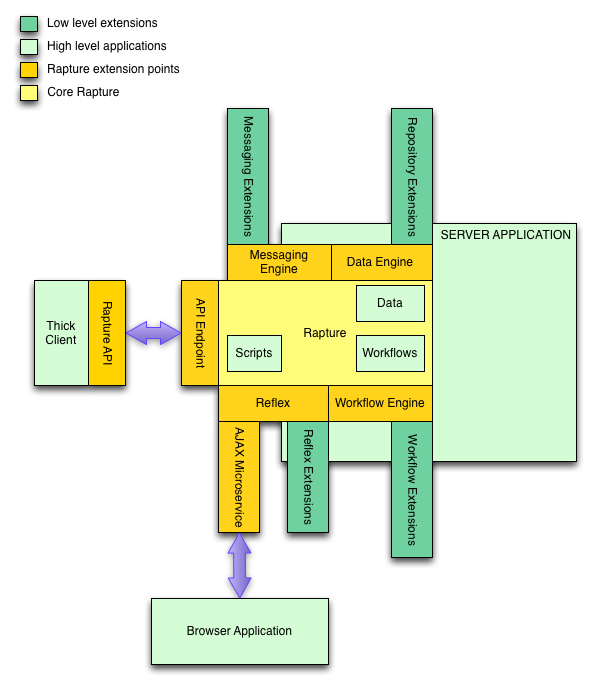
\includegraphics[scale=0.75]{Graphics/RaptureExtensionPoints}
\caption{Rapture Extension Points}
\label{fig:RaptureExtensionPoints}
\end{figure}

The diagram of Figure~\vref{fig:RaptureExtensionPoints} shows the places in which these extensions can take
place. Typically a \Rapture environment or application suite is a combination of some of these -- and Incapture Technologies
can provide some enterprise extensions (particularly in the low level extensions space) that can assist in rounding out an
application.

\section{Context and Entitlements}
Every interaction with a \Rapture API call is made in the context of a logged in
user. That user, and its entitlement group membership and the parameters passed
to the call are used to determine whether the call can proceed or not. If an
API call is used to run a script on \Rapture or to start a workflow \emph{that} script
or workflow is run in the context of the calling user as well.

In some API use categories the interface used to interact with the \Rapture API
is already bound to a user - typically this is for processes that are running
server side. Client side use cases usually have to \emph{login} to \Rapture first,
providing credentials that get translated by the \Rapture API into a \verb+CallingContext+
value (a token) which can then be used in subsequent calls to identify the user
making the call. In some client side languages there are helper constructs that
can be used to automatically pass in the logged in context to the API calls,
leaving the programmer free to not worry about this aspect.

Wrapper applications such as ReflexRunner log in on the caller's behalf and then
pass that logged in API context to the underlying container that runs the script.

\section{Custom client applications}

Client applications that talk to \Rapture can be written in any of these supported languages as
long as the application can reach (using TCP/IP) a \Rapture API Server.

\begin{itemize}
  \item{Java (or anything that runs on the Java VM and can access Java classes.)}
  \item{.NET}
  \item{Python}
  \item{Javascript (typically node.js, see a later section on architectures for browser applications.)}
  \item{Ruby}
  \item{Go(lang)}
\end{itemize}

The transport between client and server uses a JSON-RPC style of communication which
means that other language support can easily be added. The build process for
\Rapture can autogenerate client side stubs once an initial template has been
created - the authors created the .NET implementation in a few hours.

Typically the use of \Rapture in these applications follows this pattern:

\begin{enumerate}
  \item{Obtain the ip address or name of the \Rapture environment API endpoint.}
  \item{Obtain the user name and password for the use of the API.}
  \item{Call a login function to obtain a calling context.}
  \item{Pass that login context into a wrapper (for future API use) or simply pass the context into future API calls.}
\end{enumerate}

For example in Java here is a simple code extract for the login and API use process:

\begin{lstlisting}[caption={Java simple example}, language=Java]
  String host = "test.incapture.net";
  String username = "test";
  String password = "secret";
  SimpleCredentialsProvider creds = new SimpleCredentialsProvider(username, password);
  HttpLoginApi loginApi = new HttpLoginApi(host, creds);
  loginApi.login();

  ScriptClient client = new ScriptClient(loginApi);
  String content = client.getDoc().getContent("//testRepo/doc/one");
  System.out.println(content);
\end{lstlisting}

This example logs into a \Rapture environment and passes that logged in context to a \verb+ScriptClient+
instance. It is this script client that can then be easily used to interact with \Rapture. The
\verb+getContent+ call in the document API will be described in detail later.

In Python, the equivalent interaction is reproduced below:

\begin{lstlisting}[caption={Python simple example}, language=Python]
  import raptureAPI
  url = 'test.incapture.net'
  username = 'test'
  password = 'secret'
  rapture = raptureAPI.raptureAPI(url, username, password)
  content = rapture.doDoc_GetContent('//testRepo/doc/one')
  print content
\end{lstlisting}

Here we see a similar login approach and then the invocation of the same \Rapture
API call. With the same target \Rapture environment these two code snippets will
produce exactly the same output.

\section{Client Reflex scripts}

\Reflex scripts running on the client (or the server) are always running in a
container that has already been connected to an environment -- the wrapper is
the piece of code that has logged into \Rapture already.

In \Reflex then the code is even simpler. In fact \Reflex has some additional
syntax sugar for loading documents from \Rapture.

\begin{lstlisting}[caption={Reflex simple example}, language=reflex]
  contentAsMap <-- "//testRepo/doc/one";
  println(contentAsMap);

  // or

  content = #doc.getContent("//testRepo/doc/one");
  contentAsMap = fromjson(content);
  println(contentAsMap);
\end{lstlisting}

In the second access example we convert the raw JSON formatted document from
\Rapture into a \Reflex map structure so as to make the two approaches produce
the same output.

\section{Server side kernel applications}

If a Java (or Java VM) application embeds the \Rapture kernel code within it the
means for calling the \Rapture API can have a number of forms. Code running within
\Rapture has to be much more careful about calling contexts and who is actually
making the call, and there is no need to worry about host urls because the code
is running directly on \Rapture.

One approach to running the same example code is reproduced below:

\begin{lstlisting}[caption={Kernel simple example}, language=Java]
   CallingContext userContext = Kernel.getLogin().login(
          "test", "secret", null);
   String content = Kernel.getDoc().getContent(
          userContext, "//testRepo/doc/one");
   System.out.println(content);
\end{lstlisting}

Note that to run the above code your server application will have had to initialize
and configure itself first, something which is outside the scope of this document
but will trivially be a matter of defining configuration files for connection to
underlying data stores and then calling:

\begin{lstlisting}[caption={Kernel initialization}, language=Java]
   Kernel.initBootstrap();
\end{lstlisting}
